\documentclass[conference]{IEEEtran}
\IEEEoverridecommandlockouts
% The preceding line is only needed to identify funding in the first footnote. If that is unneeded, please comment it out.
\usepackage{cite}
%\usepackage{caption}
%\usepackage{subcaption}
\usepackage{amsmath,amssymb,amsfonts}
\usepackage{tikz}
\usetikzlibrary{shapes.geometric,arrows, positioning, fit, calc}
%\usepackage{algorithmic}
%\usepackage{algorithm}
%\usepackage{graphicx}
%\usepackage{xcolor}
%\usepackage{epsfig}
%\usepackage{mathptmx}
%\usepackage{textcomp}
%\usepackage{mathtools}
%\usepackage{lipsum}
%\usepackage{gensymb}

\def\BibTeX{{\rm B\kern-.05em{\sc i\kern-.025em b}\kern-.08em
    T\kern-.1667em\lower.7ex\hbox{E}\kern-.125emX}}

    \title{Project Report*\\
    {\footnotesize \textsuperscript{*}As a fulfilment to the course: "Project course name",
     D7039E \& E7032E. Lecturer: Jan van Deventer.}
    %%\thanks{Identify applicable funding agency here. If none, delete this.}
    }
    
    \author{\IEEEauthorblockN{Martin Blaszczyk, Edward Cedegård, Niklas Dahlquist, Edward Källstedt, Albin Martinsson, Måns Norell}
    \IEEEauthorblockA{\textit{Computer Science, Electrical and Space Engineering Dept.} \\
    \textit{Lule{\aa} University of Technology}\\
    Lule\aa, Sweden \\
    \{marbla-6, edwced-4, nikdah-6, edwkll-7, mnsnor-5, albmar-6\}@student.ltu.se}
    }
\date{\today}

\begin{document}
\maketitle
\begin{abstract}
\end{abstract}

\section{Introduction}
\subsection{Background and Motivation}
% Short Arrowhead introduction
Arrowhead is an initiative from Luleå University of Technology to create a unifying framework which can enable embedded devices to intergrate and interoperate services in an open-network environment. This framework and its approach will strongly conribute to the reduction of design and engineering efforts in the industry. 

% Why project course?
As part of the Engineering Project course for Master's students in Computer Science, Control and Electrical Engineering at Luleå University of Technology the goal is to implement and demonstrate how the Arrowhead Framework can be used in a factory setting using autonomous ground robots. This project report aims to give an overview of the thought process, workflows and results of the project.

The proposed solution is a robot which by implementing machine vision algorithms can navigate the factory floor while also being able to pick up object using it's arm and gripper. It utilizes the Arrowhead framework to integrate with the other parts of the model factory. 

\subsection{Contributions}
Our proposed solution is an example of how the Arrowhead framework is utilized in a scaled factory setting together with a ground robot. The design is small and modular making it easy for future imrovements and easy evaluation of the Arrowhead framework alongside third-party open-source solutions. Secondly we propose a solution consisting of lines and QR-codes and how the robot can fllow a path using a RGB-camera instead of the conventional sensors. With this camera solution the possibilities of navigating the factory floor increase compared to the basic conventional following solutions.  

\subsection{Structure}
This report in divided into...





\section*{Conceptual design}

\subsection{Mechanical structure}
The design of the robot is influenced by the LEGO\textregistered Mindstorms\textregistered EV3 set. While the original set has a movable base it was too small and without an arm with a manipulator. It also does not incorporate the Dynamixel AX-12A Smart Servos used in the final design so the decision to redesign the robot while taking design inspiration from the LEGO\textregistered EV3 design. By developing and designing a new platform it gives the possibility to adapt the dimensions and fastenings for manufacturing methods such as 3D-printing and Laser cutting. 
Consisting of seven Dynamixel\textregistered AX-12A Smart Servos for actuation, two on the base for locomotion and four on the arm and one for the gripping tool the robot has seven degrees of freedom. The main advantage of using the AX-12As is the possibility of connecting them in series which enables pararell control of all the joints. Additionaly with the built in sensors the motors return feedback of the joint angles, angular speed, current draw, teperature to name a few. 

ADD PICTURE OF CONCEPT; WRITE ABOUT THE TOP SPEED AND TURN RADIUS. ALSO HOW LONG IS THE ARM.

\subsection{Electrical components}
While the mechanical components are those visible it's the underlying electrical components that play the biggest role. The internals in the AX-12As give feedback on the state of the motors, the 1000mAh LiPo battery supplies power to the motors and surrounding electronics. For the computanions the NVIDIA\textregistered Jetson Nano is used as it runs Ubuntu natively which makes the implementation of the underlying Robotic Operating System (ROS) \cite{ros} faster.



 

\section{Project structure}


\subsection{Project planning}
The projects course started in August 2020 and continued until mid January 2020 with the project deadline in the middle of December. To have a good structre and of the things to be done and synchronizing all the parts a plan was made to have a good overview of the project, shown in Table \ref{tab:overall_time_plan}. This plan enabled the group to be eflexible while still have a good long-term structure of the project. Every month a more detailed time plan was made to facilitate the small changes, dlays etc. 
\begin{frame}
    \subsection{Time plan}
    \frametitle{Overall timetable}
    \begin{table}
        \begin{tabular}{| l | c | c | c | c }
            
            Sep & Oct & Nov & Dec \\
            \hline \hline
            Concept generation & Evaluation & Evaluation &  \\ 
            \hline
            Theory & Prototyping & Evaluation & Finishing up \\
            \hline
            Simulation & Evaluation & Evaluation & \\
            \hline
            Prototyping & Final Design & Evaluation &  \\
            \hline
 
        \end{tabular}
    \end{table}    
\end{frame}


\begin{frame}
    \frametitle{Time plan for September}
    \begin{table}
        \begin{tabular}{l | c | c | c | c }
        Subproject & Week 1 & Week 2 & Week 3 & Week 4 \\
        \hline \hline
            Arrowhead & Reading& Setup & API & Prototyping\\
            Movable base & Reading& Modeling & Simulation & Implementation\\
            Arm and grip  & Reading & Kinematics & Simulation& Prototyping\\
            Object detection & Reading & Testing & Prototyping & Evaluation\\
        \end{tabular}
    \end{table}
\end{frame}
For the group members to what task were to be done, the built in function of Issues on the souce control platform Github\textregistered \ enabled all the project group members to see what had to be done every week. A Milestone was created for each week and populated with issues. When an issue was finished it coul simply be closed. If the issue was delayed it showed clearly in the Issue overview which tasks had to be prioritized. 

\subsection{Source control}
To keep track of the different software implementation the projects souce control implements Git in one common repository \cite{repo}. The repository is where all source code and relevand 3D-files are located. This report is written in LaTeX with Git as source control. To make sure it's easy for all members to write their designated sections a workflow was designed to to minimiza merge conflicts while writing drafts as show in Fig. \ref{fig:git_workflow}. Without this flow the group members would experience merge conflicts after every push which would make it more complex and time consuming. 

    \begin{figure}
        \begin{center}
\resizebox{6.0cm}{!}{

\begin{tikzpicture}
    [align=center, auto]
    \node [computing] (start) {\textbf{CHAPTER\_descriptive\_filename.tex}};
    \node [computing, below= of start] (push) {Push to \textbf{/sections}};
    \node [computing, below= of push] (finished) {Finished?};
    \node [computing, below= of finished] (write) {Write on section}; 
    \node [computing, below= of write] (commit) {Commit};

    \node [computing, right= of finished, xshift=5em] (branch) {New branch \\ \textbf{REVIEW\_chapter}};
    \node [computing, below= of branch] (paste) {Paste section in \\ \textbf{/chapters/chapter.tex}};
    \node [computing, below= of paste] (pushb) {Push new branch};
    \node [computing, below=of pushb] (PR) {PR against \textbf{report-unsafe}};
    \node [computing, below= of PR] (review) {Wait for review};
    
    



    \coordinate [left= of push] (lrpush);
    \coordinate [left= of write] (lrwrite);
    \coordinate [left= of commit] (lrcommit);
    \coordinate [left= of finished] (lrfinished);
    \coordinate [right= of PR] (crPR);
    \coordinate [below= of crPR] (crreview);
    



    \draw [->] (commit) -- (lrcommit) -| (lrpush) -- (push);

    \draw [->] (start) -- (push);

    \draw [->] (push) -- (finished) -- node[midway, fill=white] {No} (write) -- (commit);

    \draw [->] (finished) -- node[midway, fill=white] {Yes} (branch);

    \draw [->] (branch) -- (paste) -- (pushb) -- (PR)  -- (review);

    \draw [->] (review) -| (crreview) -- node[midway, xshift=2.2em, yshift=-0.5em, fill=white] {Fix} (crPR) -- (PR);
    
    
\end{tikzpicture}
}
\end{center}
\caption{Report writing flowchart}
\label{fig:git_workflow}
\end{figure}

\begin{frame}
    \frametitle{Sequence diagram}
    \begin{figure}
        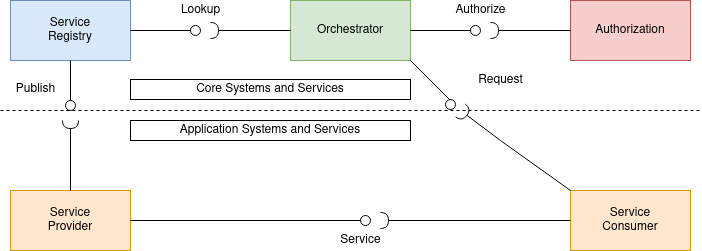
\includegraphics[width=\textwidth]{frames/images/Untitled Diagram.png}
        \end{figure}
\end{frame}

\subsection{Meetings}
The group had two weekly meetings covering the previous week and the status of the project. This structure gave the students a great deal of responsibility to do work for each meeting while still maintaining a good structure of the project and encouraged discussions. 


\bibliographystyle{IEEEtran}

\bibliography{bibliography.bib}
\end{document}





